% 若编译失败,且生成 .synctex(busy) 辅助文件,可能有两个原因:
% 1. 需要插入的图片不存在:Ctrl + F 搜索 'figure' 将这些代码注释/删除掉即可
% 2. 路径/文件名含中文或空格:更改路径/文件名即可

% --------------------- 文章宏包及相关设置 --------------------- %
% >> ------------------ 文章宏包及相关设置 ------------------ << %
% 设定文章类型与编码格式
\documentclass[UTF8]{report}		

% 本 .tex 专属的宏包
\usepackage{circledsteps} % 宏包:圆圈序号, 圆圈字母等 \Circled{1}, \CircledTop{2}
\usepackage[english]{babel} % 宏包:用于将“目录”标题换为英文 Contents

% 本 .tex 专属的宏定义、newcommand 等
    %\renewcommand{\contentsname}{目录}    % 修改目录
    % rgb(4, 9, 103), rgb(4, 10, 118)
    \definecolor{stc}{RGB}{4, 10, 118}
    \def\uV{\ \mathrm{uV}}
    \def\mV{\ \mathrm{mV}}
    \def\V{\ \mathrm{V}}
    \def\kV{\ \mathrm{KV}}
    \def\KV{\ \mathrm{KV}}
    \def\MV{\ \mathrm{MV}}
    \def\uF{\ \mathrm{uF}}
    \def\nF{\ \mathrm{nF}}
    \def\pF{\ \mathrm{pF}}
    \def\uA{\ \mathrm{uA}}
    \def\mA{\ \mathrm{mA}}
    \def\A{\ \mathrm{A}}
    \def\kA{\ \mathrm{KA}}
    \def\KA{\ \mathrm{KA}}
    \def\MA{\ \mathrm{MA}}
    \def\uO{\ \mu\Omega}
    \def\mO{\ \mathrm{m}\Omega}
    \def\O{\ \Omega}
    \def\kO{\ \mathrm{K}\Omega}
    \def\KO{\ \mathrm{K}\Omega}
    \def\MO{\ \mathrm{M}\Omega}
    \def\Hz{\ \mathrm{Hz}}
    \def\Res{\,\mathrm{Res}\,}
    \def\Im{\,\mathrm{Im}\,}
    \def\Re{\,\mathrm{Re}\,}

% 自定义宏定义
    \def\N{\mathbb{N}}
    \def\F{\mathbb{F}}
    \def\Z{\mathbb{Z}}
    \def\Q{\mathbb{Q}}
    \def\R{\mathbb{R}}
    \def\C{\mathbb{C}}
    \def\T{\mathbb{T}}
    \def\S{\mathbb{S}}
    %\def\A{\mathbb{A}}
    \def\I{\mathscr{I}}
    \def\d{\mathrm{d}}
    \def\p{\partial}


% 导入基本宏包
    \usepackage[UTF8]{ctex}     % 设置文档为中文语言
    \usepackage{hyperref}  % 宏包:自动生成超链接 (此宏包与标题中的数学环境冲突)
    \hypersetup{
        % 超链接颜色设置
        colorlinks=true,    % false:边框链接 ; true:彩色链接
        citecolor={blue},    % 文献引用颜色
        linkcolor={blue},   % 目录 (我们在目录处单独设置),公式,图表,脚注等内部链接颜色
        urlcolor={magenta},    % 网页 URL 链接颜色,包括 \href 中的 text
        % pdf 相关设置
        pdfauthor={丁毅},% PDF 作者
        pdftitle={Notes of Principles of Electric Circuits},% PDF 标题
        pdfproducer={LaTeX with hyperref}, % PDF 制作软件
        pdfcreator={xelatex},       % PDF 创建者
        pdfpagelayout=TwoColumn,    % 双栏布局
        pdfstartview=FitH,          % 页面宽度适合窗口
        %pdfpagemode=UseNone,       % 不显示书签 (默认会显示)
        pdfpagemode=UseOutlines,    % 显示书签
        pdfnewwindow=true,          % 在新窗口中打开链接
        pdfencoding=auto,           % 自动编码
        pdfborder={0 0 0},          % pdf 无边框
        pdfhighlight=/I,            % 链接高亮样式
        % magenta 洋红色
        % cyan 浅蓝色 
        % magenta 洋红色
        % yellow 黄色
        % black 黑色
        % white 白色
        % red 红色
        % green 绿色
        % blue 蓝色
        % gray 灰色
        % darkgray 深灰色
        % lightgray 浅灰色
        % brown 棕色
        % lime 石灰色
        % olive 橄榄色
        % orange 橙色
        % pink 粉红色
        % purple 紫色
        % teal 蓝绿色
        % violet 紫罗兰色
        % \textcolor{white}{白色}\
        % \textcolor{linen}{亚麻色}\​
        % \textcolor{black}{黑色}\
        % \textcolor{grey}{灰色}\
        % \textcolor{lightgrey}{浅灰色}\
        % \textcolor{darkgrey}{深灰色}\​
        % \textcolor{red}{红色}\
        % \textcolor{crimson}{深红色}\
        % \textcolor{darkred}{暗红色}\
        % \textcolor{brown}{褐色}\
        % \textcolor{maroon}{褐红色}\
        % \textcolor{salmon}{鲑红色}\
        % \textcolor{pink}{粉色}\
        % \textcolor{coral}{珊瑚色}\
        % \textcolor{orangered}{橙红色}\
        % \textcolor{orange}{橙色}\
        % ​\textcolor{blue}{蓝色}\
        % \textcolor{skyblue}{天蓝色}\
        % \textcolor{aquamarine}{海蓝色}\
        % \textcolor{navy}{深蓝色}\​
        % \textcolor{green}{绿色}\
        % \textcolor{darkgreen}{深绿色}\
        % \textcolor{seagreen}{海绿色}\
        % \textcolor{springgreen}{春绿色}\
        % \textcolor{forestgreen}{森林绿色}\
        % \textcolor{greenyellow}{绿黄色}\
        % \textcolor{yellowgreen}{黄绿色}\
        % ​\textcolor{yellow}{黄色}\
        % \textcolor{khaki}{卡其色}\
        % \textcolor{gold}{金色}\
        % \textcolor{beige}{米黄色}\
        % ​\textcolor{olive}{橄榄色}\
        % \textcolor{purple}{紫色}\
        % \textcolor{indigo}{靛青色}\
        % \textcolor{plum}{紫红色}\
        % \textcolor{violet}{紫罗兰色}\
        % \textcolor{blueviolet}{蓝紫色}\
        % \textcolor{magenta}{洋红色}\
        % ​\textcolor{cyan}{青色}\
        % \textcolor{turquoise}{青绿色}\
        % \textcolor{teal}{蓝绿色}\
        % \textcolor{tan}{棕褐色}\
    }
    % \usepackage{docmute}    % 宏包:子文件导入时自动去除导言区,用于主/子文件的写作方式,\include{./51单片机笔记}即可。注:启用此宏包会导致.tex文件capacity受限。
    \usepackage{amsmath}    % 宏包:数学公式
    \usepackage{mathrsfs}   % 宏包:提供更多数学符号
    \usepackage{amssymb}    % 宏包:提供更多数学符号
    \usepackage{pifont}     % 宏包:提供了特殊符号和字体
    \usepackage{extarrows}  % 宏包:更多箭头符号 
    \usepackage{multicol}   % 宏包:支持多栏 

% 文章页面margin设置
    \usepackage[a4paper]{geometry}
        \geometry{top=0.75in}
        \geometry{bottom=0.75in}
        \geometry{left=0.75in}
        \geometry{right=0.75in}   % 设置上下左右页边距
        \geometry{marginparwidth=1.75cm}    % 设置边注距离(注释、标记等)


% table 支持
    \usepackage{booktabs}   % 宏包:三线表
    \usepackage{tabularray} % 宏包:表格排版
    \usepackage{longtable}  % 宏包:长表格

% figure 设置
    \usepackage{graphicx}  % 支持 jpg, png, eps, pdf 图片 
    \usepackage{svg}       % 支持 svg 图片
        \svgsetup{
            % 指向 inkscape.exe 的路径
            inkscapeexe = C:/aa_MySame/inkscape/bin/inkscape.exe, 
            % 一定程度上修复导入后图片文字溢出几何图形的问题
            inkscapelatex = false                 
        }
    \usepackage{subcaption} % 用于子图和小图注  

% 图表进阶设置
    \usepackage{caption}    % 图注、表注
        \captionsetup[figure]{name=Figure}  
        \captionsetup[table]{name=Table}
        \captionsetup{
            labelfont=bf, % 设置标签为粗体
            textfont=bf,  % 设置文本为粗体
            font=small  
        }
    \usepackage{float}     % 图表位置浮动设置 
    \usepackage{etoolbox} % 用于保证图注表注的数学字符为粗体
        \AtBeginEnvironment{figure}{\boldmath} % 图注中的数学字符为粗体
        \AtBeginEnvironment{table}{\boldmath}  % 表注中的数学字符为粗体
        \AtBeginEnvironment{tabular}{\unboldmath}   % 保证表格中的数学字符不受额外影响

% 圆圈序号自定义
    \newcommand*\circled[1]{\tikz[baseline=(char.base)]{\node[shape=circle,draw,inner sep=0.8pt, line width = 0.03em] (char) {\small \bfseries #1};}}   % TikZ solution

% 列表设置
    \usepackage{enumitem}   % 宏包:列表环境设置
        \setlist[enumerate]{
            label=(\arabic*) ,   % 设置序号样式为加粗的 (1) (2) (3)
            ref=\arabic*, % 如果需要引用列表项,这将决定引用格式(这里仍然使用数字)
            itemsep=0pt, parsep=0pt, topsep=0pt, partopsep=0pt, leftmargin=3.5em} 
        \setlist[itemize]{itemsep=0pt, parsep=0pt, topsep=0pt, partopsep=0pt, leftmargin=3.5em}
        \newlist{circledenum}{enumerate}{1} % 创建一个新的枚举环境  
        \setlist[circledenum,1]{  
            label=\protect\circled{\arabic*}, % 使用 \arabic* 来获取当前枚举计数器的值,并用 \circled 包装它  
            ref=\arabic*, % 如果需要引用列表项,这将决定引用格式(这里仍然使用数字)
            itemsep=0pt, parsep=0pt, topsep=0pt, partopsep=0pt, leftmargin=3.5em
        }  

% 其它设置
    % 脚注设置
        \renewcommand\thefootnote{\ding{\numexpr171+\value{footnote}}}
    % 参考文献引用设置
        \bibliographystyle{unsrt}   % 设置参考文献引用格式为unsrt
        \newcommand{\upcite}[1]{\textsuperscript{\cite{#1}}}     % 自定义上角标式引用
    % 文章序言设置
        \newcommand{\cnabstractname}{序言}
        \newenvironment{cnabstract}{%
            \par\Large
            \noindent\mbox{}\hfill{\bfseries \cnabstractname}\hfill\mbox{}\par
            \vskip 2.0ex
            }{\par\vskip 2.5ex}
        \newcommand{\enabstractname}{Preface}
        \newenvironment{enabstract}{%
            \par\Large
            \noindent\mbox{}\hfill{\bfseries \enabstractname}\hfill\mbox{}\par
            \vskip 1.8ex
            }{\par\vskip 2.5ex}

% 文章默认字体设置
    \usepackage{fontspec}   % 宏包:字体设置
        \setmainfont{SimSun}    % 设置中文字体为宋体字体
        \setCJKmainfont[AutoFakeBold=3]{SimSun} % 设置加粗字体为 SimSun 族,AutoFakeBold 可以调整字体粗细
        \setmainfont{Times New Roman} % 设置英文字体为Times New Roman

% 各级标题自定义设置
    \usepackage{titlesec}   
        % chapter 标题自定义设置
        \titleformat{\chapter}[hang]{\normalfont\huge\bfseries\centering\boldmath\color{stc}}{Chapter\ \thechapter}{20pt}{}
        \titlespacing*{\chapter}{0pt}{-20pt}{20pt} % 控制上下间距
        % section标题自定义设置 
        \titleformat{\section}[hang]{\normalfont\Large\bfseries\boldmath\color{stc}}{\thesection}{8pt}{}
        % subsection标题自定义设置 
        \titleformat{\subsection}[hang]{\normalfont\large\bfseries\boldmath\color{stc}}{\thesubsection}{6pt}{}
        % subsubsection标题自定义设置
        \titleformat{\subsubsection}[hang]{\normalfont\bfseries\boldmath\color{stc}}{\thesubsubsection}{4pt}{}
        \titlespacing*{\subsubsection}{0pt}{3pt}{0pt} % 控制上下间距


% --------------------- 文章宏包及相关设置 --------------------- %
% >> ------------------ 文章宏包及相关设置 ------------------ << %

% ------------------------ 文章信息区 ------------------------ %
% ------------------------ 文章信息区 ------------------------ %
% 页眉页脚设置
    \usepackage{fancyhdr}   % 宏包:页眉页脚设置
        \pagestyle{fancy}
        \fancyhf{}
        \cfoot{\thepage}
        \renewcommand\headrulewidth{1pt}
        \renewcommand\footrulewidth{0pt}
        \usepackage{fontawesome}    % 宏包:更多符号与图标 (用于插入 GitHub 图标等)
        \lhead{\small
        \href{https://github.com/YiDingg/LatexNotes}{\color{black}\faGithub\ https://github.com/YiDingg/LatexNotes}
        }
        \chead{Electronic Components Manual}
        \rhead{\small dingyi233@mails.ucas.ac.cn}

%文档信息设置
    \title{电子元件手册\\ Electronic Components Manual}
    \author{丁毅\\ \footnotesize {\kaishu (中国科学院大学,北京 100049)} \\ Yi Ding \\ \footnotesize \textit{(University of Chinese Academy of Sciences, Beijing 100049, China)}}
    \date{\footnotesize 2024.11 -- ...}
% ------------------------ 文章信息区 ------------------------ %
% ------------------------ 文章信息区 ------------------------ %

% 开始编辑文章

\begin{document} 
\zihao{5}           % 设置全文字号大小

% ------------------------ 封面序言与目录 ------------------------ %
% >> --------------------- 封面序言与目录 --------------------- << %
% 封面
    \maketitle\newpage  
    \pagenumbering{Roman} % 页码为大写罗马数字
    \thispagestyle{fancy}   % 显示页码、页眉等

% 序言
\begin{cnabstract}\normalsize 
本文为笔者本科时的电子元件手册,对学习过程中接触较多的元件作了系统性的介绍和总结,同时对部分元件进行了仿真或实际电路测试,给出了相应的参数曲线或波形图。

随着学习的不断深入,笔者对某些元件的认识一定会更加深刻,也会认识新的元件。因此,笔者打算将本手册作为一份长期更新的(真的很长期)电子元件手册,既是我个人对元件知识的总结,也是便于以后自己参考。读者可到我的 GitHub 下载手册的最新版本 \href{https://github.com/YiDingg/LatexNotes}{https://github.com/YiDingg/LatexNotes},也可以在我的个人网站 \href{URL}{待更新}  上找到相关资料。

另外,有相当一部分元件(例如 Operational Amplifier)其实是基础元件所构成的模块化电路。在本书,我们不会详谈如何通过基本元件搭建出这些进阶元件,而是讨论如何对这些元件(模块化的电路)建立正确的认识,探究在不同情况下应该选用怎样的模型进行分析,以达到足够高的精度,同时尽可能地降低模型复杂度。实现它们的具体电路,以及 Oscillators、Amplifiers 和 Power Supplies 等模块化电路,会放到另一本书“电子电路手册”中,读者可到网址 \href{URL}{待更新} 自行下载和阅读。为了提高读者的自学效率,笔者在这里推荐几个免费且优秀的电子学习网站:
\begin{enumerate}
\item \href{https://www.electronics-tutorials.ws/}{Electornics Tutorials} : 这个网站提供了丰富的电子学习资料,包括 Transistors、Amplifiers、Diodes、Filters 等,还提供了很多实用的电子工程师工具,例如在线电阻电感电容计算器等;
\item \href{https://www.learnabout-electronics.org/}{Learn About Electronics} : 这个网站提供了电子学习的基础和进阶知识,包括 Semiconductors, Amplifiers, Oscillators, Power Supplies 等,最令人惊喜的是几乎所有资料都提供了 PDF 下载,方便读者下载后自行学习;
\item \href{https://www.electronics-lab.com}{Electronics Lab} : 这个网站不仅开源了很多电子电路设计实例,包括基础电路、模拟电路、数字电路等,还提供了丰富的学习资源(文章)在 \href{https://www.electronics-lab.com/articles/}{here};
\item \href{https://developerhelp.microchip.com/}{Microchip} : 这是 Microchip 官方的开发者帮助网站,提供了大量的电子元件的 Data Sheet、Application Notes、Reference Manuals 等,是学习 Microchip 产品的重要参考网站,当然,在这里也可以找到与模拟电路、数字电路相关的的学习资料;
\end{enumerate}

由于个人学识浅陋,认识有限,文中难免有不妥甚至错误之处,望读者不吝指正。读者可以将错误发送到我的邮箱 {\color{blue}\ dingyi233@mails.ucas.ac.cn},也可以到笔者的 \href{https://github.com/YiDingg/LatexNotes}{GitHub (https://github.com/YiDingg/LatexNotes)} 上提 issue,衷心感谢。

\end{cnabstract}
\addcontentsline{toc}{chapter}{序言} % 手动添加为目录




\newpage
\begin{enabstract}
    \zihao{5}
    This is an electronic components manual that I wrote during my undergraduate studies. It provide a systematic introduction and summary of the components that I encountered frequently during my studies, also includes simulations or actual circuit tests for part of the components, along with corresponding characteristics curves and waveform graphs.

    As the study progresses, my understanding of certain components will certainly become more profound, and new components will be encountered, too. Therefore, I plans to use this manual as a long-term (very long-term) electronic components manual, both as personal notes of my knowledge of components and as a reference for my reference manual in the future. Readers can freely download the latest version of the manual from my \href{https://github.com/YiDingg/LatexNotes}{  GitHub  {\color{black} (https://github.com/YiDingg/LatexNotes)}}, or find related materials on my personal website \href{URL}{to be updated}.


    Additionally, there are a considerable number of components (such as Operational Amplifier) that are actually modular circuits composed of basic components. In this book, we will not delve into how to build these advanced components using basic components, but rather discuss how to properly understand these components (modular circuits), and explore the models that should be used for analysis in different situations to achieve sufficient accuracy, while minimizing model complexity. The specific circuits for constructing these components, such as oscillators, amplifiers, power supplies etc., will be included in another book ``\textit{Electronic Circuits Manual}'', which can also be found on my GitHub \href{URL}{to be updated}. 
    
    In order to better enhance the reader's self-study efficiency, I recommends several free and excellent online learning websites here: 
    \begin{enumerate}
    \item \href{https://www.electronics-tutorials.ws}{Electornics Tutorials {\color{black} (https://www.electronics-tutorials.ws)}}: This website provides a wealth of electronic learning resources, including Transistors, Amplifiers, Diodes, Filters, and many practical tools for electronic engineers, such as an online resistor, inductor, and capacitor calculator.
    
    \item \href{https://www.learnabout-electronics.org}{  Learn About Electronics  {\color{black} (https://www.learnabout-electronics.org)}}: The website provides basic and advanced knowledge of electronics, including Semiconductors, Amplifiers, Oscillators, Power Supplies, and the best part is that almost all the materials are provided in PDF format for easy download and offline learning.
    
    \item \href{https://www.electronics-lab.com}{  Electronics Lab  {\color{black} (https://www.electronics-lab.com)}}: This website not only opensource many electronic circuit design examples, including basic circuits, analog circuits, and digital circuits, but also provides a wealth of learning resources and articles \href{https://www.electronics-lab.com/articles/}{here {\color{black} (https://www.electronics-lab.com/articles)}}.

    \item \href{https://developerhelp.microchip.com}{  Microchip  {\color{black} (https://developerhelp.microchip.com)}}: This is Microchip's official developer help website which provides a wealth of data sheets, application notes, and reference manuals for electronic components. It is an important reference website for learning about Microchip products, and of course, you can also find learning materials related to analog circuits and digital circuits here. 
\end{enumerate}
    
    Due to my own limited knowledge and understanding, there may be inappropriate or even incorrect parts in this article. I sincerely hope readers will point out any errors or inaccuracies. Readers can send errors to my email address {\color{blue} dingyi233@mails.ucas.ac.cn}, or report issues on my \href{https://github.com/YiDingg/LatexNotes}{GitHub {\color{black} (https://github.com/YiDingg/LatexNotes)}} with my utmost gratitude.
\end{enabstract}
\addcontentsline{toc}{chapter}{Preface} % 手动添加为目录



% 目录
    \setcounter{tocdepth}{2}    % 目录深度 (为 1 时显示到 section)
    % 目录页
        \tableofcontents
        \addcontentsline{toc}{chapter}{Contents}
        \thispagestyle{fancy}                   % 显示页码、页眉等
    % 插图页
        %\cleardoublepage\listoffigures
        %\addcontentsline{toc}{chapter}{插图}
        %\thispagestyle{fancy}                   % 显示页码、页眉等
    % 表格页
        %\cleardoublepage\listoftables
        %\addcontentsline{toc}{chapter}{表格}
        %\thispagestyle{fancy}                   % 显示页码、页眉等 

% 收尾工作
    \newpage    
    \pagenumbering{arabic} 


% >> --------------------- 封面序言与目录 --------------------- << %
% ------------------------ 封面序言与目录 ------------------------ %




\chapter{Resistors}\thispagestyle{fancy}


\chapter{Capacitors}\thispagestyle{fancy}

\chapter{Inductors}\thispagestyle{fancy}

\chapter{Diodes}\thispagestyle{fancy}

\section{Introduction}
Diodes are the most famous semiconductor devices, widely used in various circuits. They are made of semiconductor materials, mainly silicon (used to be selenium and germanium), and various compounds and metals are added according to the required functions.

Briefly speaking, diodes have unidirectional conductivity, allowing current to flow in only one direction.

\begin{center}
\noindent\begin{minipage}{0.55\columnwidth}
    According to different principles, diodes can be divided into the following types:
    \begin{enumerate}
    \item PN junction diode (PN 结二极管)
    \item Schottky diode (肖特基二极管)
    \item Zener diode (齐纳二极管)
    \item LED (light-emitting diode, 发光二极管)
    \item photo diode (光电二极管)
    \end{enumerate}
    According to different application scenarios (circuits), they can be roughly divided into several types:
    \begin{enumerate}
    \item rectifier diode (整流二极管)
    \item switching diode (开关二极管)
    \item regulator diode (稳压二极管)
    \item limiter diode (限幅二极管)
    \item freewheel diode (续流二极管)
    \item point contact diode (点接触二极管)
    \item LED (light-emitting diode, 发光二极管)
    \item varible capacity diode (varicap diode, 变容二极管)
    \item TVS (Transient Voltage Suppressor, 瞬态抑制二极管)
    \end{enumerate}
\end{minipage}\hfill\begin{minipage}{0.42\columnwidth}
\begin{figure}[H]\centering
    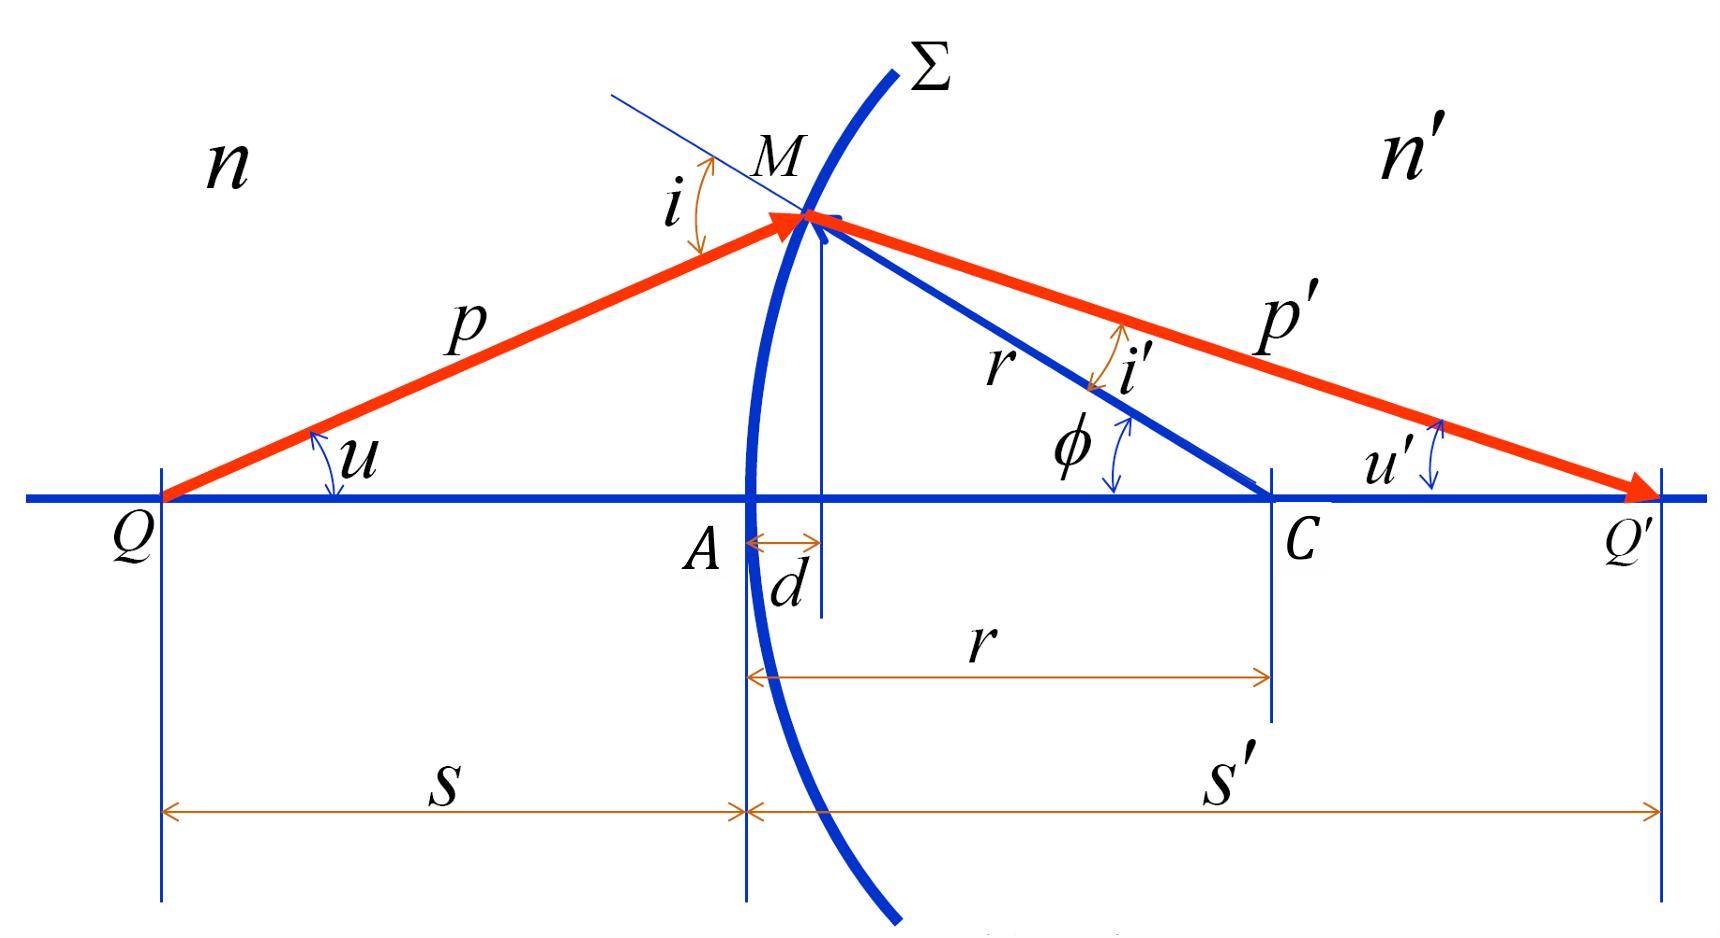
\includegraphics[width=\columnwidth]{assets/Diodes/Intro/image.png}
    \caption{Some Common Diodes}
    \label{Some Common Diodes}
\end{figure}
\end{minipage}\end{center}
Fig.\ref{Some Common Diodes} shows several common diodes, where $\Circled{1}$ are three kinds of power rectifiers, $\Circled{2}$ are small signal diodes and Zener diodes respectively, 

\section{Power/Rectifier/General Diode (功率/整流/通用二极管)}

\subsection{Concepts and Models}



\subsection{1N4007 [GOODWORK (固得沃克)]}
由 GOODWORK (固得沃克, 中国江苏) 生产的 1N4007 是一种功率/整流/通用二极管,常应用于整流电路等(同类型的有 1N4000, 1N4001, ..., 1N4006),可以在 \href{https://item.szlcsc.com/3428711.html}{立创商城} 或 \href{http://www.gk-goodwork.com/cn/product/1n4007.html}{GOODWORK 官网} 上找到它。
\begin{figure}[H]\centering
\begin{subfigure}[b]{0.5\columnwidth}\centering
    \includegraphics[height=180pt]{assets/Diodes/1N4007 [GOODWORK (固得沃克)]/1N4007 正面.png}
    \caption{The front side}
\end{subfigure}\hfill
\begin{subfigure}[b]{0.5\columnwidth}\centering
    \includegraphics[height=180pt]{assets/Diodes/1N4007 [GOODWORK (固得沃克)]/1N4007 背面.png}
    \caption{The back side}
\end{subfigure}
\caption{1N4007 [GOODWORK (固得沃克)]}
\end{figure}

Data Sheet 中的具体参数我们不再重复了,可到数据手册中自行查找。搭建测试电路如下,得到 Diodes 1N4007 的实际 I-V 工作特性如图 \ref{Operation Characteristics of 1N4007} 所示:
\begin{figure}[H]\centering
    \includegraphics[width=0.7\columnwidth]{assets/Diodes/1N4007 [GOODWORK (固得沃克)]/1N4007 Operation Chara 测试电路.pdf}
    \caption{Test Circuit for 1N4007 Operation Characteristics}
\end{figure}

\begin{figure}[H]\centering
\begin{subfigure}[b]{0.5\columnwidth}\centering
    \includegraphics[height=175pt]{assets/Diodes/1N4007 [GOODWORK (固得沃克)]/1N4007 Voltage-Current Characteristics.pdf}
    \caption{Voltage-Current Characteristics}
\end{subfigure}\hfill
\begin{subfigure}[b]{0.5\columnwidth}\centering
    \includegraphics[height=175pt]{assets/Diodes/1N4007 [GOODWORK (固得沃克)]/1N4007 Resistance Characteristics.pdf}
    \caption{Resistance Characteristics}
\end{subfigure}
\caption{Operation Characteristics of 1N4007}
\label{Operation Characteristics of 1N4007}
\end{figure}





\section{Voltage regulator diode (稳压二极管)}
\section{LED (Light Emitting Diode, 发光二极管)}
\subsection{XL-302 [XINGLIGHT (成兴光)]}
XL-302SURD (red)、XL-302SURC (white)、XL-302UYD (yellow)、XL-302UYC (green)、是由 XINGLIGHT (成兴光, 中国广东) 生产的 LED,可以在 \href{https://so.szlcsc.com/global.html?k=XL-302U}{立创商城} 或 \href{http://www.xinglight.cn/index.php?s=cpzx&c=search&keyword=XL-302}{XINGLIGHT 官网} 上找到它们。其实物图如下:

\subsection{LED [Txxbao (某宝)]}
在某宝中购买大小和外观与 XL-302 相同的 LED,其电气特性如下:
\begin{figure}[H]\centering
    \includegraphics[width=0.9\columnwidth]{assets/Diodes/LED (Taobao)/Voltage-Current Characteristics.pdf}
    \caption{Voltage-Current Characteristics}
\end{figure}
\begin{figure}[H]\centering
    \includegraphics[width=0.9\columnwidth]{assets/Diodes/LED (Taobao)/Equivalent Conductance Characteristics.pdf}
    \caption{Equivalent Conductance Characteristics}
\end{figure}
由图可以看到,黄绿红三色导通电压 $V_\text{th}$ 和 20 mA 工作压降 $V_\text{D}$ 分别为:
\begin{equation}
\boldmath
V_\text{th} = 1.8 \ \mathrm{V},\quad V_\text{D} = 2.3 \ \mathrm{V} \quad (\text{Yellow, Green, Red})
\end{equation}
而蓝色和白色 LED 的导通电压 $V_\text{th}$ 和 20 mA 工作压降 $V_\text{D}$ 分别为:
\begin{equation}
\boldmath
V_\text{th} = 2.5 \ \mathrm{V},\quad V_\text{D} = 3.2 \ \mathrm{V} \quad (\text{Blue, White})
\end{equation}

\section{Schottky Diode (肖特基二极管)}

\chapter{Transistors}\thispagestyle{fancy}
\section{BTJ (Bipolar Transistor Junction, 双极型晶体管, 三极管)}
\section{JFET (Junction Field Effect Transistor, 结型场效应晶体管)}
\section{MOSFET (Metal-Oxide -Semiconductor Field Effect Transistor, 金属氧化物半导体场效应晶体管)}


\subsection{2N7000 [onsemi (安森美)]}

2N7000 [onsemi (安森美)] 是由 onsemi 公司生产的 N-Channel Enhancement Mode Field Effect Transistor (N-Channel Enhancement MOSFET),可以在 \href{https://item.szlcsc.com/232636.html}{立创商城} 或  \href{https://www.GOODWORK.com/products/discrete-power-modules/mosfets/small-signal-mosfets/1N4007}{GOODWORK 官网} 上找到它。其实物图如下:

\begin{figure}[H]\centering
    \begin{subfigure}[b]{0.5\columnwidth}\centering
        \includegraphics[height=160pt]{assets/Transistors/2N7000 [onsemi (安森美)]/2N7000 正面.png}
        \caption{The front side}
    \end{subfigure}\hfill
    \begin{subfigure}[b]{0.5\columnwidth}\centering
        \includegraphics[height=160pt]{assets/Transistors/2N7000 [onsemi (安森美)]/2N7000 背面.png}
        \caption{The back side}
    \end{subfigure}
    \caption{2N7000 [onsemi (安森美)]}
\end{figure}


用经典反相器结构,取合适的电阻 $R_L$ 用作电流表(我们这里取 $R_L = 5.2 \Omega$),固定 $V_\text{GS}$,同时改变 $V_\text{DS}$,可以得到 MOS 的工作特性 (Operation Characteristics) $I_\text{DS} = I_\text{DS}(V_\text{DS})$,这包括了导通特性 (On-Region Characteristics) 和体二极管特性 (Body Diode Characteristics)。
\begin{figure}[H]\centering
    \includegraphics[width=0.9\columnwidth]{assets/Transistors/2N7000 [onsemi (安森美)]/2N7000 Operation Characteristics.pdf}
    \caption{Operation Characteristics of 2N7000}
\end{figure}
依据实际测得的数据,可以计算出 MOS 的等效电导特性 (Equivalent Conductance Characteristics),如下图所示:
\begin{figure}[H]\centering
    \includegraphics[width=0.9\columnwidth]{assets/Transistors/2N7000 [onsemi (安森美)]/2N7000 Cunductance Characteristics.pdf}
    \caption{Equivalent Conductance Characteristics of 2N7000}
\end{figure}
\begin{figure}[H]\centering
    \includegraphics[width=0.9\columnwidth]{assets/Transistors/2N7000 [onsemi (安森美)]/2N7000 Cunductance Characteristics (filtered).pdf}
    \caption{Filtered Equivalent Conductance Characteristics of 2N7000}
\end{figure}

固定 $V_{\text{DS}}$,改变 $V_\text{GS}$,串联万用表以测量 $I_\text{DS}$,得到 2N7000 的转移特性曲线 $I_\text{DS} = I_\text{DS}(V_\text{GS})$ 如下:
\begin{figure}[H]\centering
    \includegraphics[width=0.9\columnwidth]{assets/Transistors/2N7000 [onsemi (安森美)]/2N7000 Transfer Characteristics.pdf}
    \caption{Transfer Characteristics of 2N7000}
\end{figure}
上图中 $V_\text{DS} = 15$ V 时仅测到 $V_\text{GS} = 2.7$ V,这是因为往后 MOS 管发热严重,温度不断上升,无法得到稳定示数。用 $V_\text{DS} = 15$ V 时测得的数据拟合饱和电流公式 $I_\text{DS} = \frac{K}{2} \left( V_\text{GS} - V_\text{T} \right)^2$,其中 $K$ 和 $V_\text{T}$ 是待定参量,得到:
\begin{equation}
\boldmath V_\text{T} = 2.109 \ \mathrm{V},\quad K = 0.182 \ \mathrm{A\cdot V^{-2}} = 182 \ \mathrm{mA\cdot V^{-2}}
\end{equation}

\begin{figure}[H]\centering
    \includegraphics[width=0.9\columnwidth]{assets/Transistors/2N7000 [onsemi (安森美)]/2N7000 拟合 K 值与 V_T.png}
    \caption{Threshold Voltage of 2N7000}
\end{figure}

\subsection{FinFET (Fin Field-Effect Transistor, 鳍式场效应晶体管)}

\section{MODFET (Modulationdoped Field-Effect Transistor, 调制掺杂场效应晶体管) }
\section{Darlington Transistors (达林顿晶体管)}

\chapter{Amplifiers}\thispagestyle{fancy}
\section{Common Emitter Amplifier (共射极放大器)}
\section{Common Base Amplifier (共基极放大器)}
\section{Common Collector Amplifier (共集极放大器)}
\section{Common Source Amplifier (共源极放大器)}
\section{MOSFET Amplifier (MOSFET 放大器)}

\subsection{LM258P}
\subsection{NE5532P}
\subsection{LM318N}

\section{Class AB Amplifier (AB 类放大器)}

\chapter{}\thispagestyle{fancy}



















\end{document}



% VScode 常用快捷键:

% F2:                       变量重命名
% Ctrl + Enter:             行中换行
% Alt + up/down:            上下移行
% 鼠标中键 + 移动:           快速多光标
% Shift + Alt + up/down:    上下复制
% Ctrl + left/right:        左右跳单词
% Ctrl + Backspace/Delete:  左右删单词    
% Shift + Delete:           删除此行
% Ctrl + J:                 打开 VScode 下栏(输出栏)
% Ctrl + B:                 打开 VScode 左栏(目录栏)
% Ctrl + `:                 打开 VScode 终端栏
% Ctrl + 0:                 定位文件
% Ctrl + Tab:               切换已打开的文件(切标签)
% Ctrl + Shift + P:         打开全局命令(设置)

% Latex 常用快捷键

% Ctrl + Alt + J:           由代码定位到PDF
% 


% Git提交规范:
% update: Linear Algebra 2 notes
% add: Linear Algebra 2 notes
% import: Linear Algebra 2 notes
% delete: Linear Algebra 2 notes